% Options for packages loaded elsewhere
\PassOptionsToPackage{unicode}{hyperref}
\PassOptionsToPackage{hyphens}{url}
%
\documentclass[
  ignorenonframetext,
  aspectratio=169,
]{beamer}
\usepackage{pgfpages}
\setbeamertemplate{caption}[numbered]
\setbeamertemplate{caption label separator}{: }
\setbeamertemplate{navigation symbols}{}
\setbeamertemplate{footline}[page number]
\setbeamertemplate{itemize item}{\small\raise0.5pt\hbox{$\bullet$}}
\setbeamertemplate{itemize subitem}{\tiny\raise1.5pt\hbox{$\bullet$}}
\setbeamertemplate{itemize subsubitem}{\tiny\raise1.5pt\hbox{$\bullet$}}
\setbeamercolor{caption name}{fg=normal text.fg}
\beamertemplatenavigationsymbolsempty
% Prevent slide breaks in the middle of a paragraph
\widowpenalties 1 10000
\raggedbottom
\setbeamertemplate{part page}{
  \centering
  \begin{beamercolorbox}[sep=16pt,center]{part title}
    \usebeamerfont{part title}\insertpart\par
  \end{beamercolorbox}
}
\setbeamertemplate{section page}{
  \centering
  \begin{beamercolorbox}[sep=12pt,center]{part title}
    \usebeamerfont{section title}\insertsection\par
  \end{beamercolorbox}
}
\setbeamertemplate{subsection page}{
  \centering
  \begin{beamercolorbox}[sep=8pt,center]{part title}
    \usebeamerfont{subsection title}\insertsubsection\par
  \end{beamercolorbox}
}
\AtBeginPart{
  \frame{\partpage}
}
\AtBeginSection{
  \ifbibliography
  \else
    \frame{\sectionpage}
  \fi
}
\AtBeginSubsection{
  \frame{\subsectionpage}
}
\usepackage{amsmath,amssymb}
\usepackage{lmodern}
\usepackage{iftex}
\ifPDFTeX
  \usepackage[T1]{fontenc}
  \usepackage[utf8]{inputenc}
  \usepackage{textcomp} % provide euro and other symbols
\else % if luatex or xetex
  \ifXeTeX
    \usepackage{xltxtra} 
    \usepackage{xeCJK}
    \setCJKmainfont{ipaexm.ttf}
    \setCJKsansfont{ipaexg.ttf}
    \setCJKmonofont{ipaexg.ttf}
  \fi
  \usepackage{unicode-math}
  \defaultfontfeatures{Scale=MatchLowercase}
  \defaultfontfeatures[\rmfamily]{Ligatures=TeX,Scale=1}
\fi
% Use upquote if available, for straight quotes in verbatim environments
\IfFileExists{upquote.sty}{\usepackage{upquote}}{}
\IfFileExists{microtype.sty}{% use microtype if available
  \usepackage[]{microtype}
  \UseMicrotypeSet[protrusion]{basicmath} % disable protrusion for tt fonts
}{}
\makeatletter
\@ifundefined{KOMAClassName}{% if non-KOMA class
  \IfFileExists{parskip.sty}{%
    \usepackage{parskip}
  }{% else
    \setlength{\parindent}{0pt}
    \setlength{\parskip}{6pt plus 2pt minus 1pt}}
}{% if KOMA class
  \KOMAoptions{parskip=half}}
\makeatother
\usepackage{xcolor}
\IfFileExists{xurl.sty}{\usepackage{xurl}}{} % add URL line breaks if available
\IfFileExists{bookmark.sty}{\usepackage{bookmark}}{\usepackage{hyperref}}
\hypersetup{
  pdftitle={Estimating Effect of Tax Incentives on Charitable Giving Considering Self-Selection of Tax Relief in South Korea},
  hidelinks,
  pdfcreator={LaTeX via pandoc}}
\urlstyle{same} % disable monospaced font for URLs

\usepackage{setspace}
\usepackage{float}

\newif\ifbibliography
\usepackage{longtable,booktabs,array}
\usepackage{threeparttable, threeparttablex, multirow}
\usepackage{calc} % for calculating minipage widths
\usepackage{caption}
% Make caption package work with longtable
\makeatletter
\def\fnum@table{\tablename~\thetable}
\makeatother
\usepackage{graphicx}
\makeatletter
\def\maxwidth{\ifdim\Gin@nat@width>\linewidth\linewidth\else\Gin@nat@width\fi}
\def\maxheight{\ifdim\Gin@nat@height>\textheight\textheight\else\Gin@nat@height\fi}
\makeatother
% Scale images if necessary, so that they will not overflow the page
% margins by default, and it is still possible to overwrite the defaults
% using explicit options in \includegraphics[width, height, ...]{}
\setkeys{Gin}{width=\maxwidth,height=\maxheight,keepaspectratio}
% Set default figure placement to htbp
\makeatletter
\def\fps@figure{htbp}
\makeatother
\setlength{\emergencystretch}{3em} % prevent overfull lines
\providecommand{\tightlist}{%
  \setlength{\itemsep}{0pt}\setlength{\parskip}{0pt}}
\setcounter{secnumdepth}{-\maxdimen} % remove section numbering
\newlength{\cslhangindent}
\setlength{\cslhangindent}{1.5em}
\newlength{\csllabelwidth}
\setlength{\csllabelwidth}{3em}
\newlength{\cslentryspacingunit} % times entry-spacing
\setlength{\cslentryspacingunit}{\parskip}
\newenvironment{CSLReferences}[2] % #1 hanging-ident, #2 entry spacing
 {% don't indent paragraphs
  \setlength{\parindent}{0pt}
  % turn on hanging indent if param 1 is 1
  \ifodd #1
  \let\oldpar\par
  \def\par{\hangindent=\cslhangindent\oldpar}
  \fi
  % set entry spacing
  \setlength{\parskip}{#2\cslentryspacingunit}
 }%
 {}
\usepackage{calc}
\newcommand{\CSLBlock}[1]{#1\hfill\break}
\newcommand{\CSLLeftMargin}[1]{\parbox[t]{\csllabelwidth}{#1}}
\newcommand{\CSLRightInline}[1]{\parbox[t]{\linewidth - \csllabelwidth}{#1}\break}
\newcommand{\CSLIndent}[1]{\hspace{\cslhangindent}#1}


\ifLuaTeX
  \usepackage{selnolig}  % disable illegal ligatures
\fi

\title{Estimating Effect of Tax Incentives on Charitable Giving Considering Self-Selection of Tax Relief in South Korea  }
\author[shortname]{ Hiroki Kato \inst{1} \and  Tsuyoshi Goto \inst{2} \and  Yong-Rok Kim \inst{3} \and }
\institute[shortinst]{ \inst{1} Osaka University \and  \inst{2} Chiba University \and  \inst{3} Kansai University \and }

\date{2022/01/05}


\begin{document}
\frame{\titlepage}

\begin{frame}{社会にとって寄付の税インセンティブを与えることは望ましいか?}
\protect\hypertarget{ux793eux4f1aux306bux3068ux3063ux3066ux5bc4ux4ed8ux306eux7a0eux30a4ux30f3ux30bbux30f3ux30c6ux30a3ux30d6ux3092ux4e0eux3048ux308bux3053ux3068ux306fux671bux307eux3057ux3044ux304b}{}
\begin{itemize}
\tightlist
\item
  多くの国の税制は、所得控除や税額控除を通して、寄付に金銭的インセンティブを設けている

  \begin{itemize}
  \tightlist
  \item
    利点: 公共財の私的供給を促進する
  \item
    欠点: 税収を減らしてしまう
  \end{itemize}
\item
  税収の減少分を十分に上回るだけの寄付を増やせれば、税インセンティブは社会的に望ましい

  \begin{itemize}
  \tightlist
  \item
    厚生評価の重要なパラメータ: 寄付の(税)価格弾力性
  \item
    この絶対値が1を超えれば、税インセンティブは社会的に望ましい (Saez, 2004)
  \end{itemize}
\item
  韓国の税制改革を用いて、寄付の価格弾力性を推定することを目的とする
\end{itemize}
\end{frame}

\begin{frame}{税インセンティブの自己選択の問題}
\protect\hypertarget{ux7a0eux30a4ux30f3ux30bbux30f3ux30c6ux30a3ux30d6ux306eux81eaux5df1ux9078ux629eux306eux554fux984c}{}
税インセンティブと申告コストに基づいて、納税者は控除を受けるかどうかを意思決定する

\begin{itemize}
\tightlist
\item
  申告コストが大きいことを指摘している研究がいくつかある

  \begin{itemize}
  \tightlist
  \item
    アメリカの個人所得税の確定申告: 申告準備(Record keeping)のコスト \textgreater{} 申告自体(Tax filing)のコスト (Benzarti, 2020)
  \item
    イギリスの寄付控除の固定費用: 申告された寄付額の10\%に相当 (Almunia et al., 2020)
  \item
    デンマークの寄付控除でも、record keepingのコストを含めた様々なoptimization frictionがある (Gillitzer and Skov, 2018)
  \end{itemize}
\item
  韓国においても、寄付控除を受けるためのコストは大きいと考えられる

  \begin{itemize}
  \tightlist
  \item
    控除を受けた寄付者の割合は42\% (from our data)
  \item
    控除を受けた寄付者の平均寄付額は174万ウォンである一方、控除を受けていない寄付者の平均寄付額は133万ウォン (from our data)
  \end{itemize}
\end{itemize}
\end{frame}

\begin{frame}{本研究の概要(1)}
\protect\hypertarget{ux672cux7814ux7a76ux306eux6982ux89811}{}
韓国における2014年の税制改革を用いて、税インセンティブの自己選択を考慮した寄付の価格弾力性を推定する

\begin{itemize}
\tightlist
\item
  韓国のパネルデータ(National Survey of Tax and Benefit)を使用する

  \begin{itemize}
  \tightlist
  \item
    サーベイデータの利点 \(\to\) 申告された寄付額は実際の寄付額と異なる測定誤差(Fack and Landais, 2016; Gillitzer and Skov, 2018)を回避できる
  \end{itemize}
\item
  2014年の税制改革(所得控除 \(\to\) 税額控除)を税インセンティブの外生変動として利用したDIDで推定する

  \begin{itemize}
  \tightlist
  \item
    所得税率に依存したインセンティブ(所得控除)から納税者に一律のインセンティブ(税額控除)に変更
  \end{itemize}
\item
  申告コストの外生要因として、給与所得者かどうかを用いる

  \begin{itemize}
  \tightlist
  \item
    給与所得者はそれ以外よりも申告コストが低いと予想される
  \end{itemize}
\end{itemize}
\end{frame}

\begin{frame}{本研究の概要(2)}
\protect\hypertarget{ux672cux7814ux7a76ux306eux6982ux89812}{}
Result

\begin{enumerate}
\tightlist
\item
  Baseline results show that the giving price elasticity is less than -1.4 in terms of intensive margins and less than -1.7 in terms of extensive margins in Korea.
\item
  The estimated giving price elasticity for those who declare charitable giving is around -1.2 -1.6.

  \begin{itemize}
  \tightlist
  \item
    These estimates are more elastic than the estimates in the extant research, many of which show around -1.
  \end{itemize}
\item
  By reducing application cost, we can increase charitable giving.
\item
  Given our estimates, increasing the subsidy on charitable giving will be desirable in Korea.
\end{enumerate}
\end{frame}

\hypertarget{ux97d3ux56fdux306eux5bc4ux4ed8ux63a7ux9664ux5236ux5ea6}{%
\section{韓国の寄付控除制度}\label{ux97d3ux56fdux306eux5bc4ux4ed8ux63a7ux9664ux5236ux5ea6}}

\begin{frame}{寄付控除のモデル}
\protect\hypertarget{ux5bc4ux4ed8ux63a7ux9664ux306eux30e2ux30c7ux30eb}{}
\begin{align}
  x_{it} + g_{it} = y_{it} - R_{it}T_t(y_{it}, g_{it}) - (1 - R_{it}) T_t(y_{it})
\end{align}

\begin{itemize}
\tightlist
\item
  \(x_{it}\)は私的消費財、\(g_{it}\)は寄付額
\item
  \(y_{it}\)は課税前所得、\(R_{it}\)は寄付を申告するかどうかのダミー変数
\item
  \(T_t(y_{it})\)と\(T_t(y_{it}, g_{it})\)は寄付申告をしなかったときの課税額と申告したときの課税額
\item
  寄付の税インセンティブは\(s_{it} = \partial T_t(y_{it}, g_{it}) / \partial g_{it}\)であり、寄付の相対価格は\(1 - s_{it}\)
\end{itemize}

\((g_{it}, y_{it})\)を所与として、寄付控除の節税額が申告コスト(\(K_{it}\))を上回るとき、寄付控除を受ける

\begin{align}
  R_{it} = 1[T_t(y_{it}) - T_t(y_{it}, g_{it}) > K_{it}]
\end{align}
\end{frame}

\begin{frame}{2014年の税制改革: 所得控除から税額控除へ}
\protect\hypertarget{ux5e74ux306eux7a0eux5236ux6539ux9769-ux6240ux5f97ux63a7ux9664ux304bux3089ux7a0eux984dux63a7ux9664ux3078}{}
所得控除 (income deduction)

\begin{align}
  T_t(y_{it}, g_{it}) = T_t(y_{it} - g_{it})
\end{align}

\begin{itemize}
\tightlist
\item
  税インセンティブは\(s_{it} = T'_t(y_{it} - g_{it})\)
\item
  高所得であるほど税負担が軽減される(限界税率が高い)ので、低所得より高所得の方が有利な制度
\end{itemize}

税額控除(tax credit)

\begin{align}
  T_t(y_{it}, g_{it}) = T_t(y_{it}) - m g_{it}
\end{align}

\begin{itemize}
\tightlist
\item
  \(m\)は税額控除率であり、\(m = 0.15\) \(\to\) 税インセンティブは\(s_{it} = m\)
\item
  2014年の税制改革は税の逆進性を緩和し、税負担の公平性を改善することを目的として、所得に依存しない均一なインセンティブを導入した (Fig. \ref{fig:SummaryPrice})
\end{itemize}
\end{frame}

\begin{frame}{韓国における寄付申告の手続き}
\protect\hypertarget{ux97d3ux56fdux306bux304aux3051ux308bux5bc4ux4ed8ux7533ux544aux306eux624bux7d9aux304d}{}
韓国では所得税納税者は寄付に対して税制上の優遇を受けることができる

\begin{itemize}
\tightlist
\item
  優遇を受けるためには、1年間の寄付の証明書を提出して寄付申告する必要がある

  \begin{itemize}
  \tightlist
  \item
    給与所得者と非給与所得者で手続きが大きく異なる
  \end{itemize}
\item
  給与所得者

  \begin{itemize}
  \tightlist
  \item
    所得税を源泉徴収で納税し、寄付申告は会社で行う
  \item
    給与所得者は証明書の提出は随時行うことができる
  \item
    控除制度の正しい理解や書類作成の必要は特にない
  \end{itemize}
\item
  非給与所得者

  \begin{itemize}
  \tightlist
  \item
    所得納税を確定申告で行い、寄付申告は確定申告時に国税庁で行う
  \item
    確定申告は翌年の5月に実施
  \item
    確定申告時まで証明書を保存しておく必要がある \(\to\) 寄付証明書の発行をめぐり、寄付団体に5月頃問い合わせが殺到
  \item
    確定申告時には寄付金控除を受けるための申請書類を作成する必要がある
  \end{itemize}
\item
  給与所得者のほうが寄付の申告コスト(\(K_{it}\))が低いと考えられる (Fig. \ref{fig:SummaryReliefbyEarner})
\end{itemize}
\end{frame}

\hypertarget{ux30c7ux30fcux30bf}{%
\section{データ}\label{ux30c7ux30fcux30bf}}

\begin{frame}{National Survey of Tax and Benefit (NaSTaB)}
\protect\hypertarget{national-survey-of-tax-and-benefit-nastab}{}
\begin{itemize}
\tightlist
\item
  2008年からKorea Institute of Taxation and Financeが実施
\item
  NaSTaBは家計の税負担や公的扶助などに関する年次パネルデータ
\item
  全国から5,634世帯を調査対象とする

  \begin{itemize}
  \tightlist
  \item
    5,634人の世帯主と15歳以上で経済活動をしている世帯員が調査に回答する
  \end{itemize}
\item
  我々の研究では(1)2013年から2018年かつ、(2)23歳以下の回答者を除いたデータを使用する

  \begin{itemize}
  \tightlist
  \item
    2012年と2013年の所得税率は変化していないが、2011年以前に所得税率の改正が何度か行われた (Table \ref{tab:TaxRate})
  \item
    2014年の制度改革に着目するために、2013年から2018年に限定する
  \item
    23歳以下の回答者は所得や資産を十分に持っていない可能性が高いので、データから除外する
  \end{itemize}
\end{itemize}
\end{frame}

\begin{frame}{Descriptive Statistics}
\protect\hypertarget{descriptive-statistics}{}
\begin{table}

\caption{\label{tab:SummaryCovariate}Descriptive Statistics}
\centering
\fontsize{6}{8}\selectfont
\begin{tabular}[t]{lcccccc}
\toprule
  & N & Mean & Std.Dev. & Min & Median & Max\\
\midrule
\addlinespace[0.3em]
\multicolumn{7}{l}{\textbf{Income and giving price}}\\
\hspace{1em}Annual taxable labor income (unit: 10,000KRW) & 36189 & 1747.26 & 2696.77 & 0.00 & 0.00 & 50000.00\\
\hspace{1em}First giving relative price & 36198 & 0.86 & 0.04 & 0.62 & 0.85 & 0.94\\
\addlinespace[0.3em]
\multicolumn{7}{l}{\textbf{Charitable giving}}\\
\hspace{1em}Annual chariatable giving (unit: 10,000KRW) & 36199 & 35.64 & 153.20 & 0.00 & 0.00 & 10000.00\\
\hspace{1em}Dummary of donation > 0 & 36199 & 0.24 & 0.42 & 0.00 & 0.00 & 1.00\\
\hspace{1em}Dummy of declaration of a tax relief & 36199 & 0.10 & 0.30 & 0.00 & 0.00 & 1.00\\
\addlinespace[0.3em]
\multicolumn{7}{l}{\textbf{Individual Characteristics}}\\
\hspace{1em}Age & 36199 & 53.45 & 16.22 & 24.00 & 51.00 & 103.00\\
\hspace{1em}Female dummy & 36199 & 0.43 & 0.50 & 0.00 & 0.00 & 1.00\\
\hspace{1em}University graduate & 36198 & 0.42 & 0.49 & 0.00 & 0.00 & 1.00\\
\hspace{1em}High school graduate dummy & 36198 & 0.31 & 0.46 & 0.00 & 0.00 & 1.00\\
\hspace{1em}Junior high school graduate dummy & 36198 & 0.27 & 0.44 & 0.00 & 0.00 & 1.00\\
\hspace{1em}Wage earner dummy & 27394 & 0.56 & 0.50 & 0.00 & 1.00 & 1.00\\
\hspace{1em}\#.Tax accountant / population & 36199 & 1.04 & 0.51 & 0.32 & 0.92 & 2.24\\
\bottomrule
\end{tabular}
\end{table}
\end{frame}

\begin{frame}{右歪曲の所得分布と寄付価格の変動}
\protect\hypertarget{ux53f3ux6b6aux66f2ux306eux6240ux5f97ux5206ux5e03ux3068ux5bc4ux4ed8ux4fa1ux683cux306eux5909ux52d5}{}
\begin{figure}[t]

{\centering 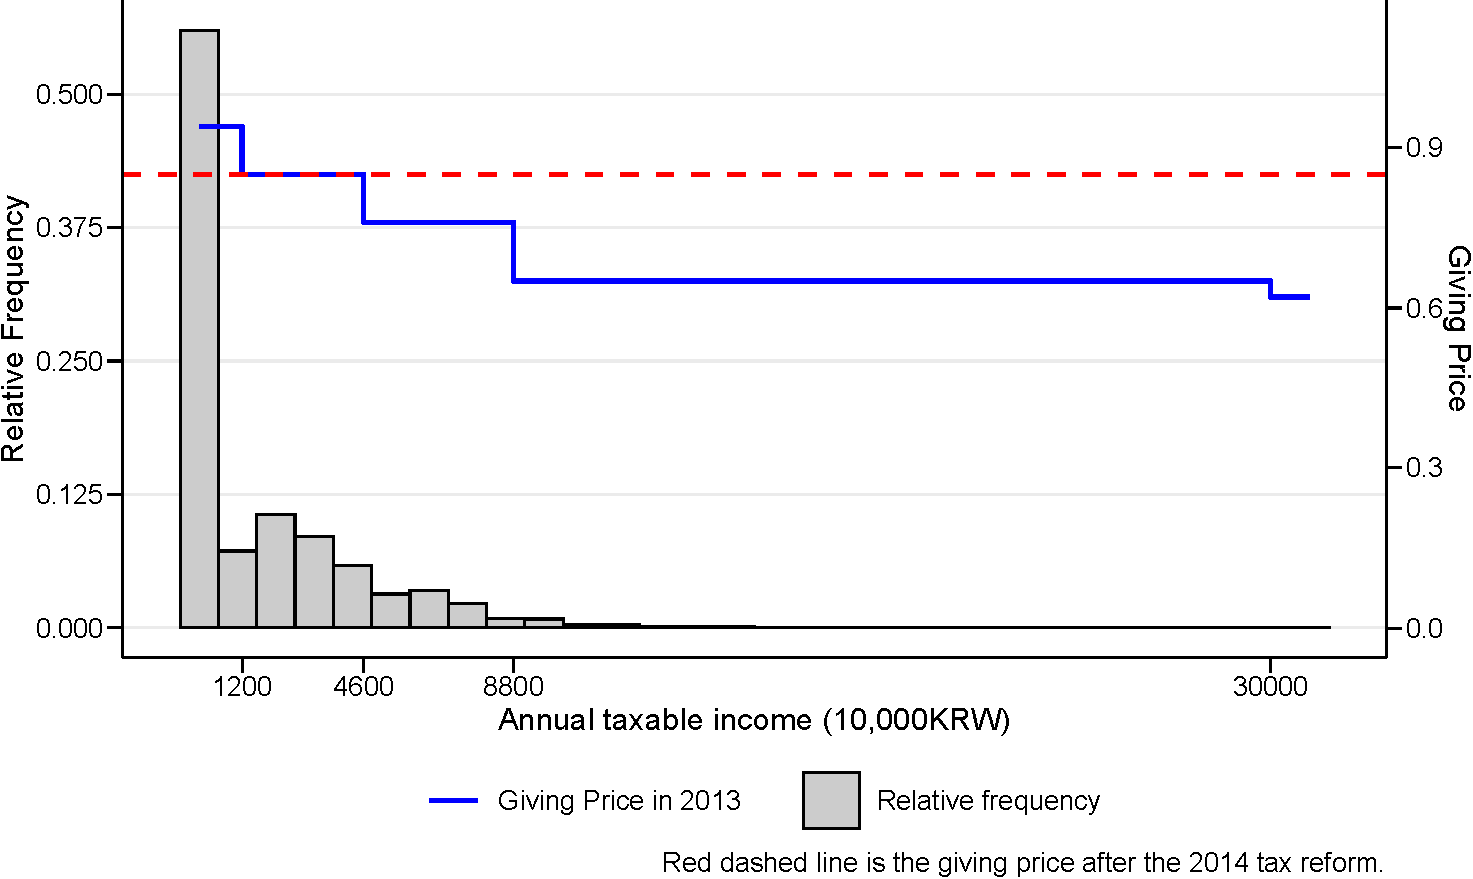
\includegraphics[width=0.7\linewidth,]{C:/Users/katoo/Desktop/NASTAB/paper/slide_files/figure-beamer/SummaryPrice-1} 

}

\caption{Income Distribution in 2013 and Relative Giving Price. Notes: The left and right axis measure the relative frequency of respondents (grey bars) and the relative giving price (solid step line and dashed line), respectively. A solid step line and a dashed horizontal line represents the giving price in 2013 and 2014, respectively.}\label{fig:SummaryPrice}
\end{figure}
\end{frame}

\begin{frame}{2014年税制改革直後、寄付者比率が減少}
\protect\hypertarget{ux5e74ux7a0eux5236ux6539ux9769ux76f4ux5f8cux5bc4ux4ed8ux8005ux6bd4ux7387ux304cux6e1bux5c11}{}
\begin{figure}[t]

{\centering 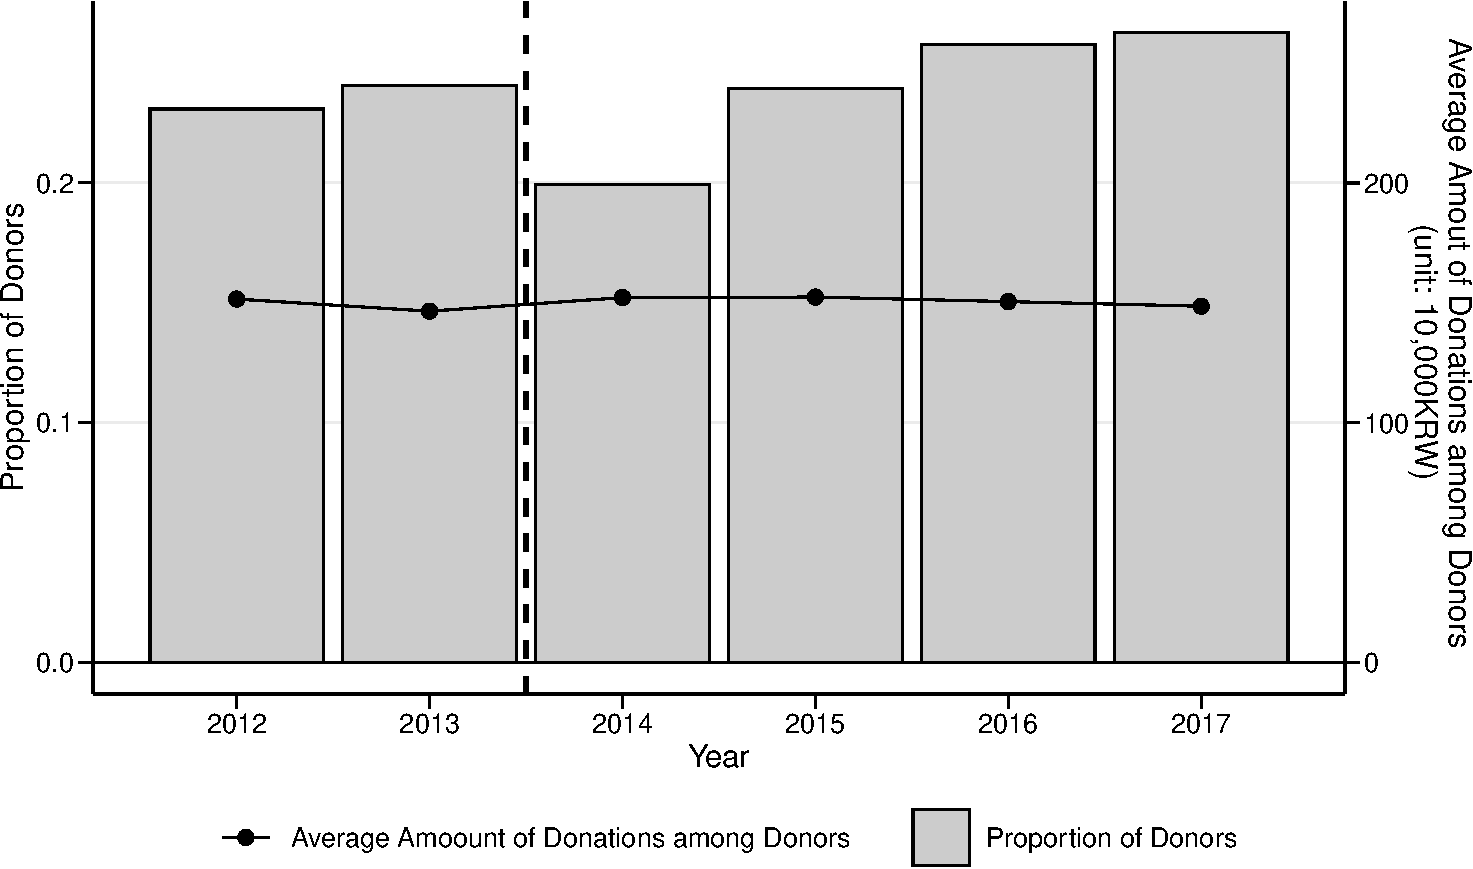
\includegraphics[width=0.7\linewidth,]{C:/Users/katoo/Desktop/NASTAB/paper/slide_files/figure-beamer/SummaryGiving-1} 

}

\caption{Proportion of Donors and Average Donations among Donors. Notes: The left and right axises measure prooortion of donors (grey bars) and the average amount of donations among donors (solid line), respectively.}\label{fig:SummaryGiving}
\end{figure}
\end{frame}

\begin{frame}{税インセンティブは寄付額を増やした}
\protect\hypertarget{ux7a0eux30a4ux30f3ux30bbux30f3ux30c6ux30a3ux30d6ux306fux5bc4ux4ed8ux984dux3092ux5897ux3084ux3057ux305f}{}
\begin{figure}[t]

{\centering 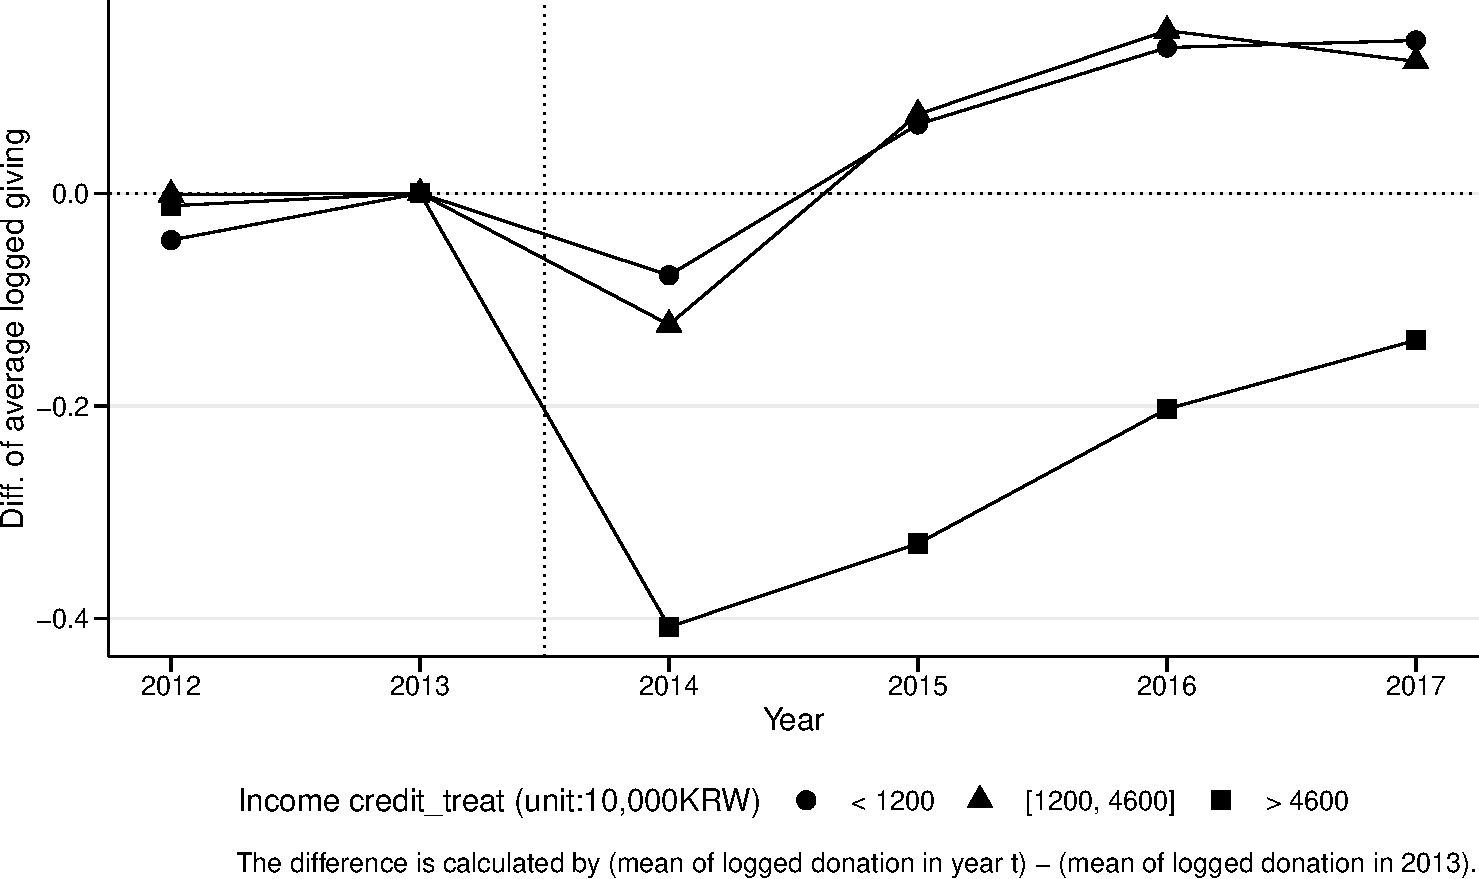
\includegraphics[width=0.7\linewidth,]{C:/Users/katoo/Desktop/NASTAB/paper/slide_files/figure-beamer/SummaryGivingOverall-1} 

}

\caption{Average Logged Giving by Three Income Groups. Notes: We created three income groups, with the relative price of giving rising (circle), unchanged (triangle), and falling (square) between 2013 and 2014. The group averages are normalized to be zero in 2013.}\label{fig:SummaryGivingOverall}
\end{figure}
\end{frame}

\begin{frame}{寄付者に限定すると、寄付額に対する価格効果ははっきりとしない}
\protect\hypertarget{ux5bc4ux4ed8ux8005ux306bux9650ux5b9aux3059ux308bux3068ux5bc4ux4ed8ux984dux306bux5bfeux3059ux308bux4fa1ux683cux52b9ux679cux306fux306fux3063ux304dux308aux3068ux3057ux306aux3044}{}
\begin{figure}[t]

{\centering 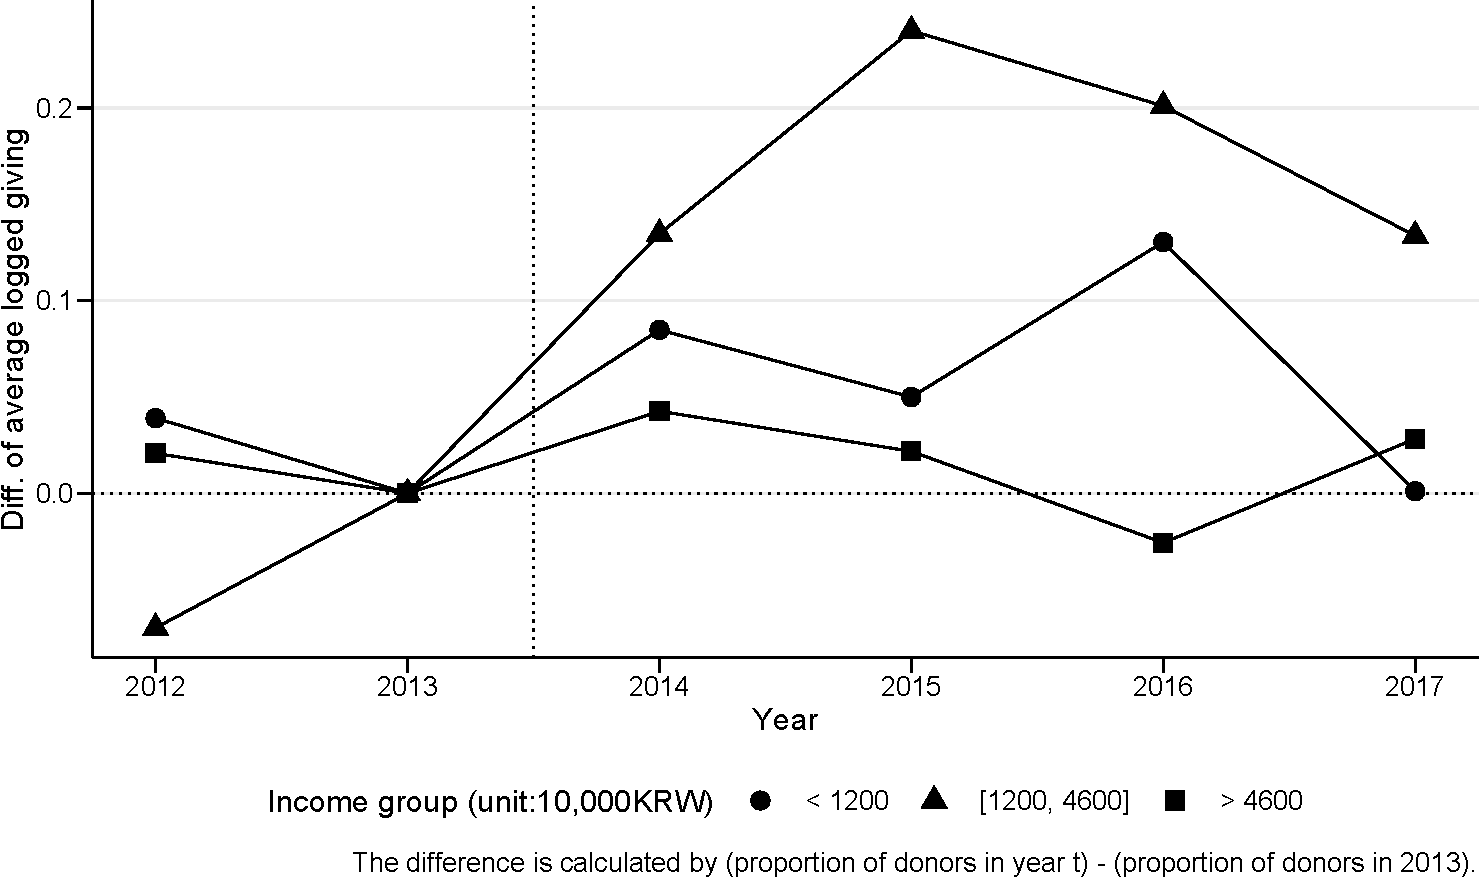
\includegraphics[width=0.7\linewidth,]{C:/Users/katoo/Desktop/NASTAB/paper/slide_files/figure-beamer/SummaryGivingIntensive-1} 

}

\caption{Average Logged Giving by Three Income Groups Conditional on Donors. Notes: We created three income groups, with the relative price of giving rising (circle), unchanged (triangle), and falling (square) between 2013 and 2014. The group averages are normalized to be zero in 2013.}\label{fig:SummaryGivingIntensive}
\end{figure}
\end{frame}

\begin{frame}{税インセンティブは寄付者を増やした}
\protect\hypertarget{ux7a0eux30a4ux30f3ux30bbux30f3ux30c6ux30a3ux30d6ux306fux5bc4ux4ed8ux8005ux3092ux5897ux3084ux3057ux305f}{}
\begin{figure}[t]

{\centering 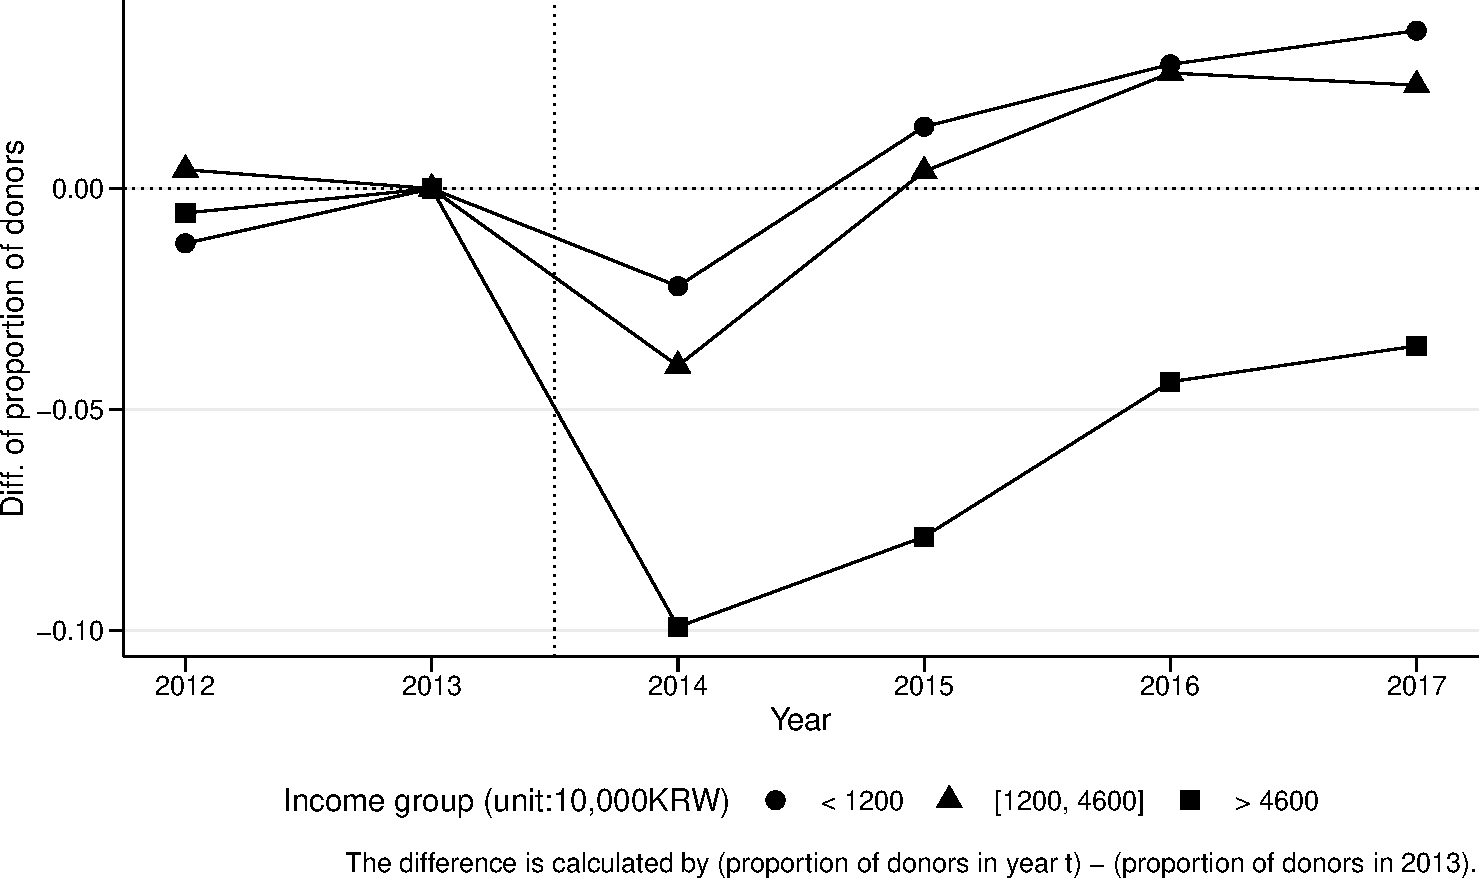
\includegraphics[width=0.7\linewidth,]{C:/Users/katoo/Desktop/NASTAB/paper/slide_files/figure-beamer/SummaryGivingExtensive-1} 

}

\caption{Proportion of Donors by Three Income Groups. Notes: We created three income groups, with the relative price of giving rising (circle), unchanged (triangle), and falling (square) between 2013 and 2014. The group averages are normalized to be zero in 2013.}\label{fig:SummaryGivingExtensive}
\end{figure}
\end{frame}

\begin{frame}{制度改革に関わらず、給与所得者は寄付申告をしやすい}
\protect\hypertarget{ux5236ux5ea6ux6539ux9769ux306bux95a2ux308fux3089ux305aux7d66ux4e0eux6240ux5f97ux8005ux306fux5bc4ux4ed8ux7533ux544aux3092ux3057ux3084ux3059ux3044}{}
\begin{figure}[t]

{\centering 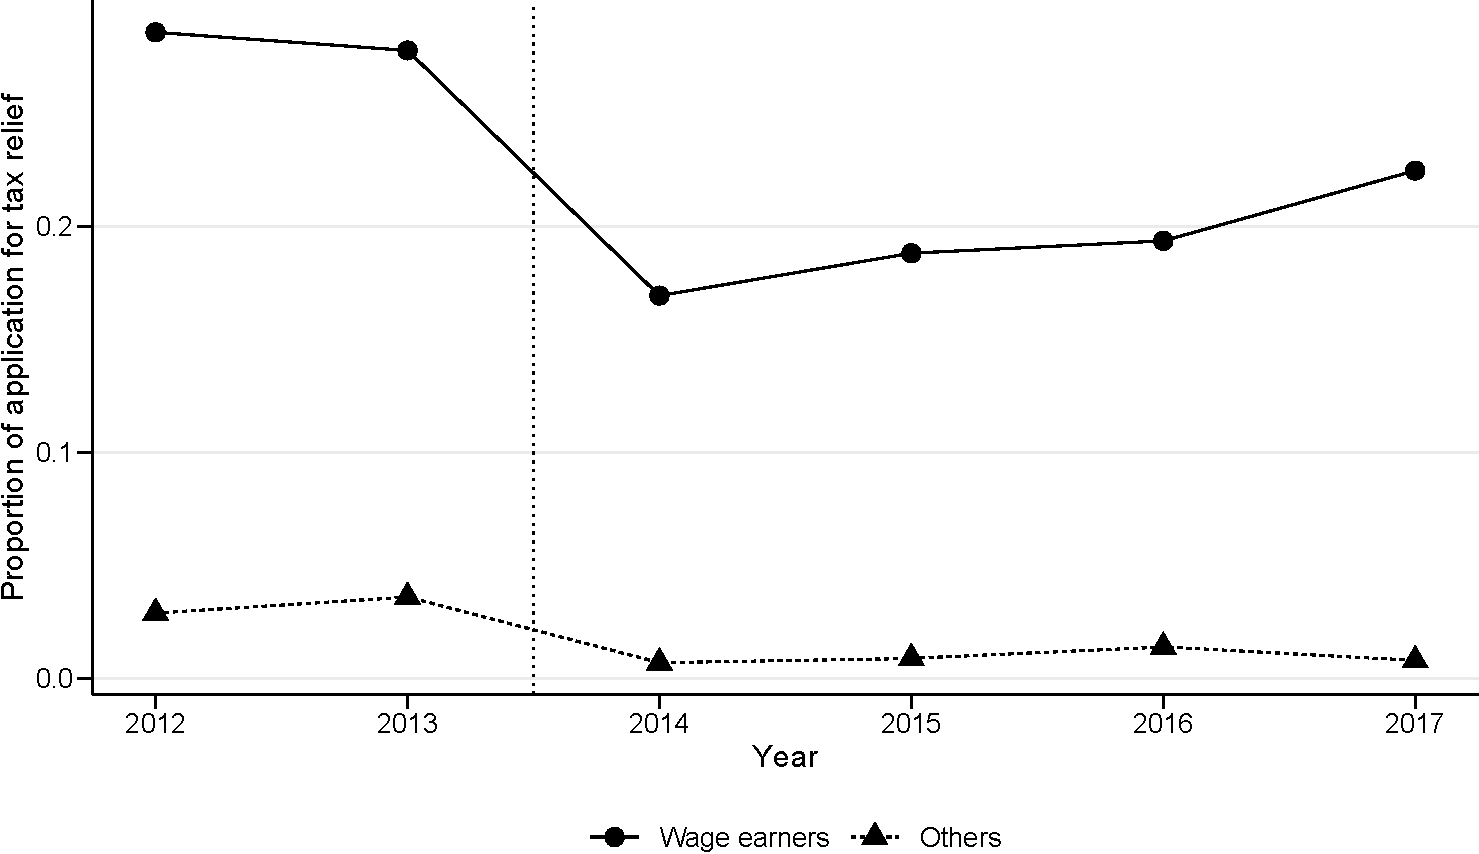
\includegraphics[width=0.7\linewidth,]{C:/Users/katoo/Desktop/NASTAB/paper/slide_files/figure-beamer/SummaryReliefbyEarner-1} 

}

\caption{Share of Tax Relief by Wage Earners. Notes: A solid line is the share of applying for tax relief among wage eaners. A dashed line is the share of applying for tax relief other than wage earners.}\label{fig:SummaryReliefbyEarner}
\end{figure}
\end{frame}

\hypertarget{ux5bc4ux4ed8ux306eux4fa1ux683cux5f3eux529bux6027ux306eux63a8ux5b9a}{%
\section{寄付の価格弾力性の推定}\label{ux5bc4ux4ed8ux306eux4fa1ux683cux5f3eux529bux6027ux306eux63a8ux5b9a}}

\begin{frame}{2種類の寄付の価格弾力性}
\protect\hypertarget{ux7a2eux985eux306eux5bc4ux4ed8ux306eux4fa1ux683cux5f3eux529bux6027}{}
Almunia et al. (2020) に従い、2種類の価格弾力性を推定する

\begin{enumerate}
\tightlist
\item
  Intensive-margin tax-price elasticity: 1\%の価格上昇で寄付者の寄付額が何\%増えるか?
\item
  Extensive-margin tax-price elasticity: 1\%の価格上昇で寄付確率が何\%増えるか?
\end{enumerate}
\end{frame}

\begin{frame}{Intensive-Margin Tax-Price Elasticityの推定方法}
\protect\hypertarget{intensive-margin-tax-price-elasticityux306eux63a8ux5b9aux65b9ux6cd5}{}
\begin{align}
  \ln g_{it} = \theta_i + \gamma (R_{it} \times \ln (1 - s_{it}))
  + \beta X_{it} + \lambda_t + u_{it}, \label{eq:intensive}
\end{align}

\begin{itemize}
\tightlist
\item
  \(X_{it}\)は課税前所得(\(y_{it}\))を含んだ共変量ベクトル
\item
  \(\theta_i\)は個人固定効果、\(\lambda_t\)は時間固定効果
\item
  \(u_{it}\)はidiosyncratic error
\item
  関心のあるパラメータは\(\gamma\)で、intensive-margin tax-price elasticityを示す
\end{itemize}
\end{frame}

\begin{frame}{Extensive-Margin Tax-Price Elasticityの推定方法}
\protect\hypertarget{extensive-margin-tax-price-elasticityux306eux63a8ux5b9aux65b9ux6cd5}{}
\begin{align}
  D_{it} = \theta_i + \delta (R_{it} \times \ln (1 - s_{it}))
  + \beta X_{it} + \lambda_t + u_{it}, \label{eq:extensive}
\end{align}

\begin{itemize}
\tightlist
\item
  \(D_{it}\)は正の寄付額(\(g_{it} > 0\))が観測されたら1を取るダミー変数
\item
  関心のあるパラメータは\(\delta\)

  \begin{itemize}
  \tightlist
  \item
    二値のアウトカム変数なので、\(\delta\)は直接、価格弾力性として解釈できない
  \item
    Extensive-Margin Tax-Price Elasticityは\(\hat{\delta} / \bar{D}\)で得られる(\(\bar{D}\)は\(D_{it}\)の標本平均)
  \end{itemize}
\end{itemize}
\end{frame}

\begin{frame}{寄付の相対価格の内生性}
\protect\hypertarget{ux5bc4ux4ed8ux306eux76f8ux5bfeux4fa1ux683cux306eux5185ux751fux6027}{}
\begin{align}
  1 - s_{it} =
  \begin{cases}
    1 - T'_t(y_{it} - g_{it})  \quad\text{if}\quad t < 2014  \\
    1 - m \quad\text{if}\quad t \ge 2014
  \end{cases},
\end{align}

\begin{itemize}
\tightlist
\item
  \(T'_t(\cdot)\)は\(t\)年の限界所得税率、\(m\)は税額控除率(\(m = 0.15\))
\item
  所得控除のとき、寄付価格は寄付額(\(g_{it}\))に依存する
\item
  この価格は\emph{Last}-unit priceと呼ばれる
\end{itemize}

過去の研究にならい、本研究は以下の\emph{first}-unit priceを\emph{last}-unit priceの代わり(もしくはその操作変数)として用いる

\begin{align}
  1 - s^f_{it} =
  \begin{cases}
    1 - T'_t(y_{it} - 0)  \quad\text{if}\quad t < 2014  \\
    1 - m \quad\text{if}\quad t \ge 2014
  \end{cases},
\end{align}
\end{frame}

\begin{frame}{寄付申告の内生性}
\protect\hypertarget{ux5bc4ux4ed8ux7533ux544aux306eux5185ux751fux6027}{}
給与所得者ダミーをexclusionとして用いる

\begin{itemize}
\tightlist
\item
  所得や業種をコントロールすれば、給与所得者であるかどうかは直接寄付額に影響しない
\item
  給与所得者のほうが非給与所得者より寄付申告コストが安いと考えられる
\end{itemize}

Wooldridge (2010) より、以下の二つの方法で推定する

\begin{enumerate}
\tightlist
\item
  給与所得者ダミー(\(Z_{it}\))とfirst-unit priceの交差項を\(R_{it} \times \ln (1 - s^f_{it})\)の操作変数として用いる
\item
  寄付申告の傾向スコア\(P_{it}\)とfirst-unit priceの交差項を操作変数として用いる

  \begin{itemize}
  \tightlist
  \item
    傾向スコア\(P_{it}\)は\(R_{it} = 1[\alpha_0 + \alpha_1 Z_{it} + \alpha_2 \ln(1 - s^f_{it}) + \alpha_3 X_{it} + u_{it0} > 0]\)をプロビット推定し、その予測確率で得る
  \item
    プロビット推定は係数が時間に対して一定と仮定したPooledモデルと係数が時間に対して異なると仮定したSeparatedモデルで推定
  \end{itemize}
\end{enumerate}
\end{frame}

\begin{frame}{結果: Intensive-Margin Tax-Price Elasticity}
\protect\hypertarget{ux7d50ux679c-intensive-margin-tax-price-elasticity}{}
\begin{table}

\caption{\label{tab:MainIntensive}Intensive-Margin Tax-Price Elasticity}
\centering
\fontsize{7}{9}\selectfont
\begin{threeparttable}
\begin{tabular}[t]{lcccccc}
\toprule
\multicolumn{1}{c}{ } & \multicolumn{3}{c}{FE} & \multicolumn{3}{c}{FE-2SLS} \\
\cmidrule(l{3pt}r{3pt}){2-4} \cmidrule(l{3pt}r{3pt}){5-7}
  & (1) & (2) & (3) & (4) & (5) & (6)\\
\midrule
Applying tax relief x log(first price) & -0.748*** &  &  & -1.400*** & -1.437*** & -1.540***\\
 & (0.225) &  &  & (0.411) & (0.363) & (0.375)\\
PS of applying tax relief x log(first price) &  & -1.544*** & -1.515*** &  &  & \\
 &  & (0.388) & (0.367) &  &  & \\
\midrule
First-stage: Instrument &  &  &  & 0.638 & 1.075 & 0.984\\
 &  &  &  & [468.1] & [534.6] & [662.2]\\
Num.Obs. & 7004 & 6975 & 6975 & 6975 & 6975 & 6975\\
Instrument &  &  &  & WE x Price & PS x Price & PS x Price\\
Method of PS &  & Pool & Separate &  & Pool & Separate\\
\bottomrule
\end{tabular}
\begin{tablenotes}
\item Notes: $^{*}$ $p < 0.1$, $^{**}$ $p < 0.05$, $^{***}$ $p < 0.01$. Standard errors are clustered at individual level. A square bracket is wald statistics of instrument.
\end{tablenotes}
\end{threeparttable}
\end{table}
\end{frame}

\begin{frame}{結果: Extensive-Margin Tax-Price Elasticity}
\protect\hypertarget{ux7d50ux679c-extensive-margin-tax-price-elasticity}{}
\begin{table}

\caption{\label{tab:MainExtensive}Extensive-Margin Tax-Price Elasticity}
\centering
\fontsize{7}{9}\selectfont
\begin{threeparttable}
\begin{tabular}[t]{lcccccc}
\toprule
\multicolumn{1}{c}{ } & \multicolumn{3}{c}{FE} & \multicolumn{3}{c}{FE-2SLS} \\
\cmidrule(l{3pt}r{3pt}){2-4} \cmidrule(l{3pt}r{3pt}){5-7}
  & (1) & (2) & (3) & (4) & (5) & (6)\\
\midrule
Applying tax relief x log(first price) & -2.800*** &  &  & -0.464*** & -0.563*** & -0.738***\\
 & (0.074) &  &  & (0.176) & (0.120) & (0.116)\\
PS of applying tax relief x log(first price) &  & -0.452*** & -0.566*** &  &  & \\
 &  & (0.107) & (0.101) &  &  & \\
\midrule
Implied price elasticity & -10.799*** & -1.741*** & -2.181*** & -1.788*** & -2.169*** & -2.841***\\
 & (0.287) & (0.411) & (0.388) & (0.678) & (0.463) & (0.448)\\
First-stage: Instrument &  &  &  & 0.289 & 0.803 & 0.768\\
 &  &  &  & [276.6] & [311.7] & [361.9]\\
Num.Obs. & 27017 & 26863 & 26863 & 26863 & 26863 & 26863\\
Instrument &  &  &  & WE x Price & PS x Price & PS x Price\\
Method of PS &  & Pool & Separate &  & Pool & Separate\\
\bottomrule
\end{tabular}
\begin{tablenotes}
\item Notes: $^{*}$ $p < 0.1$, $^{**}$ $p < 0.05$, $^{***}$ $p < 0.01$. Standard errors are clustered at individual level. A square bracket is wald statistics of instrument.
\end{tablenotes}
\end{threeparttable}
\end{table}
\end{frame}

\begin{frame}{ロバストネスチェック}
\protect\hypertarget{ux30edux30d0ux30b9ux30c8ux30cdux30b9ux30c1ux30a7ux30c3ux30af}{}
\begin{enumerate}
\tightlist
\item
  2013-2014年データを除外 (Table \ref{tab:WoAnnoucementIntensive} and \ref{tab:WoAnnouncementExtensive})

  \begin{itemize}
  \tightlist
  \item
    税制改革のアナウンスメント効果を排除
  \end{itemize}
\item
  First-unit priceではなく、Last-unit priceで弾力性を推定 (Table \ref{tab:LastIntensive} and \ref{tab:LastExtensive})
\item
  給与所得者ダミーと寄付価格の交差項ではなく、first-unit priceを操作変数にする (Table \ref{tab:MainElasticity}-\ref{tab:WoAnnoucementElasticity})
\item
  寄付申告者に限定し、所得控除制度による内生性(e.g.~所得の変動)を考慮した分析を実施 (Table \ref{tab:R1Elasticity} and \ref{tab:KdiffElasticity})

  \begin{itemize}
  \tightlist
  \item
    階差モデルやリードラグ変数の使用 (Almunia et al., 2020; Gruber and Saez, 2002; Randolph, 1995)
  \end{itemize}
\end{enumerate}

ほとんどの分析で、intensive-margin tax-price elasticityは-1.5から-2の間に入り、
extensive-margin tax-price elasticityは-1.7から-5の間に入る
\end{frame}

\begin{frame}{韓国での寄付の価格弾力性は先行研究より弾力的}
\protect\hypertarget{ux97d3ux56fdux3067ux306eux5bc4ux4ed8ux306eux4fa1ux683cux5f3eux529bux6027ux306fux5148ux884cux7814ux7a76ux3088ux308aux5f3eux529bux7684}{}
\begin{itemize}
\tightlist
\item
  申告の自己選択を無視すると、Intensive-margin tax-price elasticityは過小推定

  \begin{itemize}
  \tightlist
  \item
    寄付者の寄付額を決める観察できない要素と申告が正の相関をしている
  \item
    そのような要素を寄付額を高めるならば、節税による便益が高くなるので、申告しやすくなる
  \end{itemize}
\item
  申告の自己選択を無視すると、Extensive-margin tax-price elasticityは過大推定

  \begin{itemize}
  \tightlist
  \item
    寄付価格が申告と寄付するかどうかの意思決定の両方に同じ方向の影響を与え、負の相関をより強くした可能性がある
  \end{itemize}
\end{itemize}
\end{frame}

\hypertarget{primitive-result-marginal-treatment-effect}{%
\section{(Primitive Result) Marginal Treatment Effect}\label{primitive-result-marginal-treatment-effect}}

\begin{frame}{線型のMTE関数}
\protect\hypertarget{ux7ddaux578bux306emteux95a2ux6570}{}
\begin{center}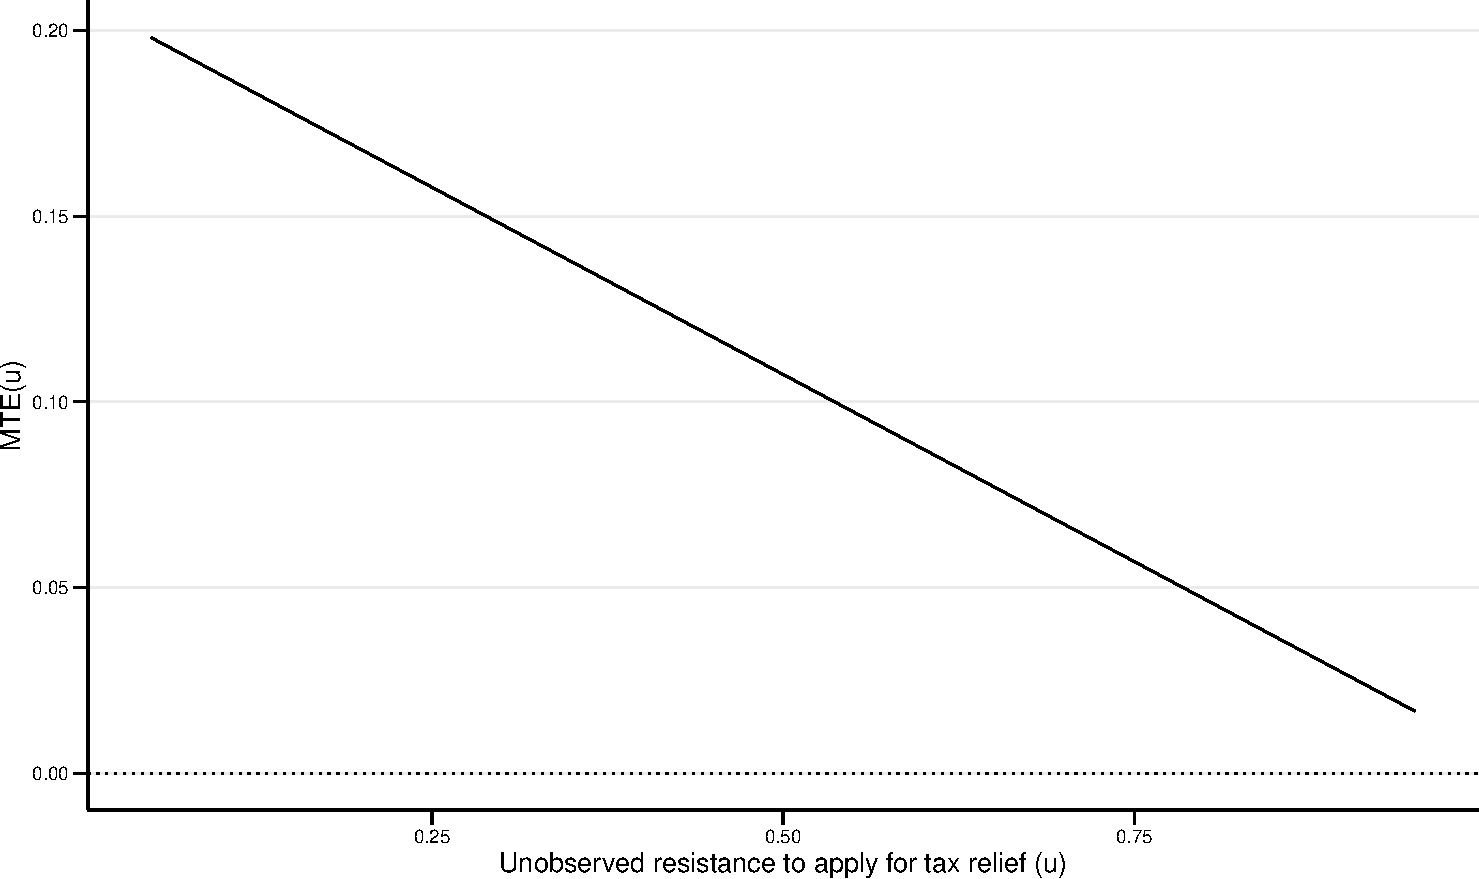
\includegraphics[width=0.7\linewidth]{C:/Users/katoo/Desktop/NASTAB/paper/slide_files/figure-beamer/unnamed-chunk-22-1} \end{center}
\end{frame}

\begin{frame}{Population-levelパラメータの推定}
\protect\hypertarget{population-levelux30d1ux30e9ux30e1ux30fcux30bfux306eux63a8ux5b9a}{}
\begin{table}

\caption{\label{tab:unnamed-chunk-23}Estimating ATE, ATU and ATT on logged donations}
\centering
\fontsize{7}{9}\selectfont
\begin{tabular}[t]{lccc}
\toprule
Target & Estimated Effect & Mean of Logged Price & Implied Elasticity\\
\midrule
ATT & 0.1352 & -0.1886 & -0.7167\\
ATE & 0.1301 & -0.1645 & -0.7909\\
ATU & 0.1247 & -0.1466 & -0.8506\\
\bottomrule
\end{tabular}
\end{table}
\end{frame}

\hypertarget{conclusion}{%
\section{Conclusion}\label{conclusion}}

\hypertarget{appendix}{%
\section{Appendix}\label{appendix}}

\begin{frame}{所得税率の変遷}
\protect\hypertarget{ux6240ux5f97ux7a0eux7387ux306eux5909ux9077}{}
\begin{table}

\caption{\label{tab:TaxRate}Marginal Income Tax Rate}
\centering
\fontsize{9}{11}\selectfont
\begin{threeparttable}
\begin{tabular}[t]{lccccccc}
\toprule
Income/Year & 2008 & 2009 & 2010 \textasciitilde{} 2011 & 2012 \textasciitilde{} 2013 & 2014 \textasciitilde{} 2016 & 2017 & 2018\\
\midrule
(A) \textasciitilde{} 1200 & 8\% & 6\% & 6\% & 6\% & 6\% & 6\% & 6\%\\
\cmidrule{1-8}
(B) 1200 \textasciitilde{} 4600 & 17\% & 16\% & 15\% & 15\% & 15\% & 15\% & 15\%\\
\cmidrule{1-8}
(C) 4600 \textasciitilde{} 8800 & 26\% & 25\% & 24\% & 24\% & 24\% & 24\% & 24\%\\
\cmidrule{1-8}
(D) 8800 \textasciitilde{} 15000 &  &  &  &  & 35\% &  & 35\%\\
\cmidrule{1-1}
\cmidrule{6-6}
\cmidrule{8-8}
(E) 15000 \textasciitilde{} 30000 &  &  &  & \multirow{-2}{*}{\centering\arraybackslash 35\%} &  & \multirow{-2}{*}{\centering\arraybackslash 35\%} & 38\%\\
\cmidrule{1-1}
\cmidrule{5-5}
\cmidrule{7-8}
(F) 30000 \textasciitilde{} 50000 &  &  &  &  &  & 38\% & 40\%\\
\cmidrule{1-1}
\cmidrule{7-8}
(G) 50000 \textasciitilde{} & \multirow{-4}{*}{\centering\arraybackslash 35\%} & \multirow{-4}{*}{\centering\arraybackslash 35\%} & \multirow{-4}{*}{\centering\arraybackslash 35\%} & \multirow{-2}{*}{\centering\arraybackslash 38\%} & \multirow{-3}{*}{\centering\arraybackslash 38\%} & 40\% & 42\%\\
\bottomrule
\end{tabular}
\begin{tablenotes}
\item Notes: Marginal income tax rates applied from 2008 to 2018 are summarized. The income level is shown in terms of 10,000 KRW, which is approximately 10 United States dollars (USD) at an exchange rate of 1,000 KRW to one USD.
\end{tablenotes}
\end{threeparttable}
\end{table}
\end{frame}

\begin{frame}{Distribution of Donations Conditional on Donors}
\protect\hypertarget{distribution-of-donations-conditional-on-donors}{}
\begin{figure}[t]

{\centering 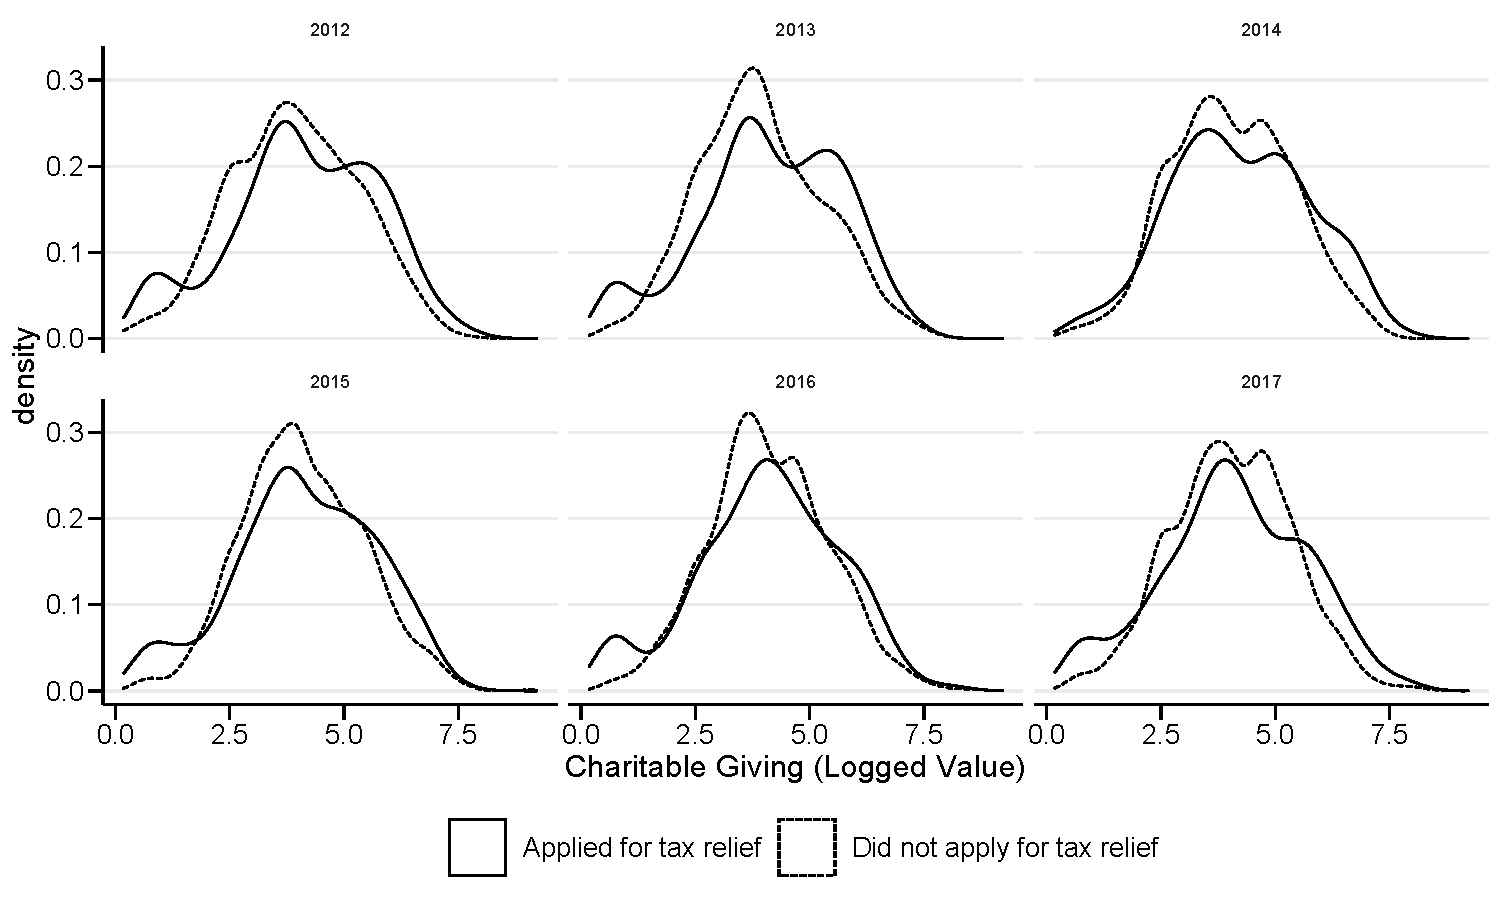
\includegraphics[width=0.7\linewidth,]{C:/Users/katoo/Desktop/NASTAB/paper/slide_files/figure-beamer/SummaryGivingIntensiveDist-1} 

}

\caption{Distribution of Charitable Giving among Those Who Donated}\label{fig:SummaryGivingIntensiveDist}
\end{figure}
\end{frame}

\begin{frame}{Share of Application Conditional on Donors by Wage Earners}
\protect\hypertarget{share-of-application-conditional-on-donors-by-wage-earners}{}
\begin{figure}[t]

{\centering 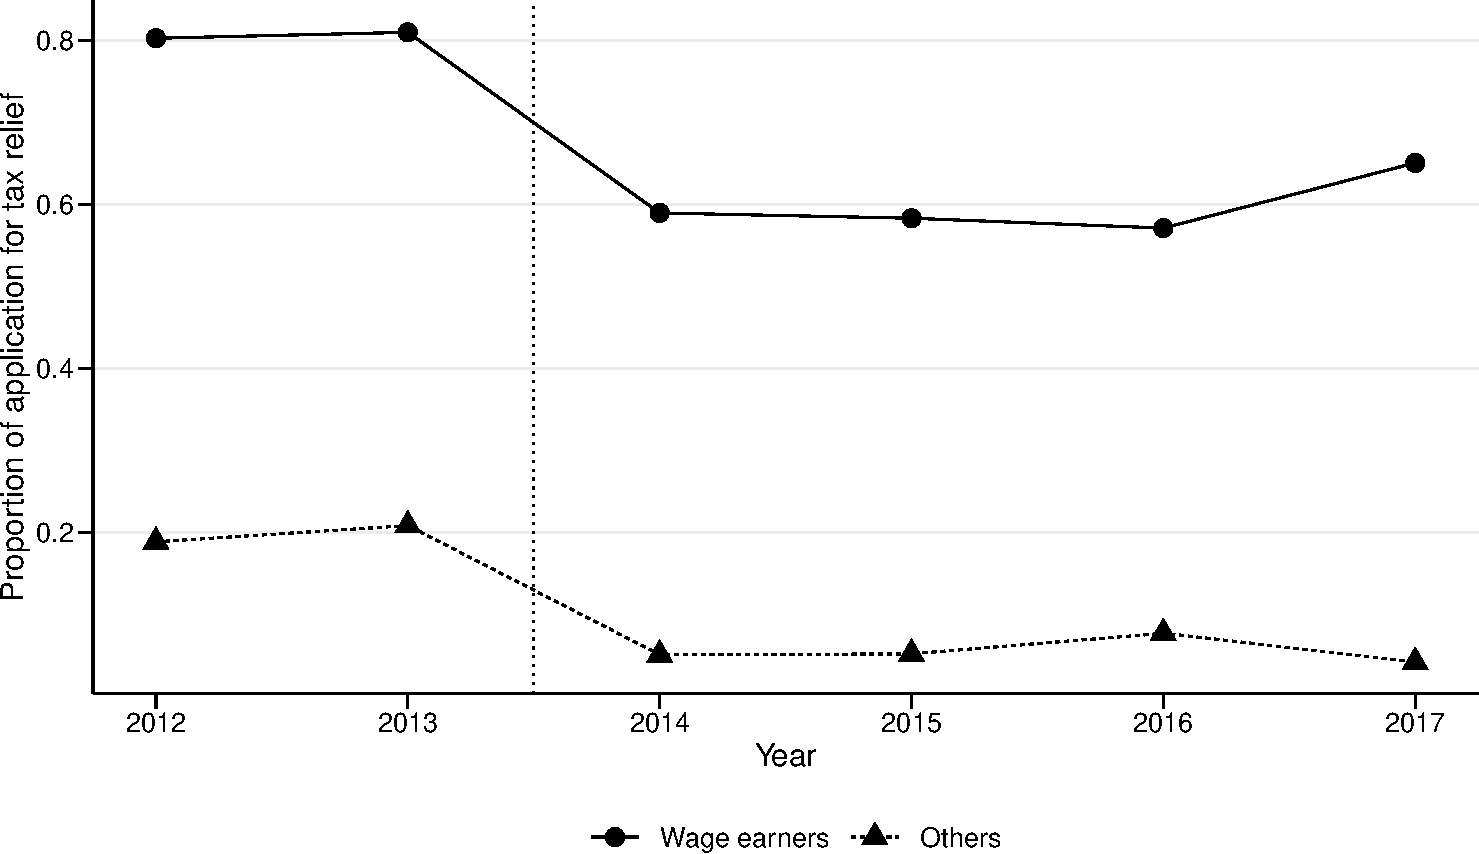
\includegraphics[width=0.7\linewidth,]{C:/Users/katoo/Desktop/NASTAB/paper/slide_files/figure-beamer/SummaryReliefbyEarner2-1} 

}

\caption{Share of Tax Relief by Wage Earners Conditional on Donors. Notes: A solid line is the share of applying for tax relief among wage eaners. A dashed line is the share of applying for tax relief other than wage earners.}\label{fig:SummaryReliefbyEarner2}
\end{figure}
\end{frame}

\begin{frame}{Intensive-Margin Tax-Price Elasticity w/o Announcement Effect}
\protect\hypertarget{intensive-margin-tax-price-elasticity-wo-announcement-effect}{}
\begin{table}

\caption{\label{tab:WoAnnoucementIntensive}Intensive-Margin Tax-Price Elasticity Excluding 2013 and 2014 data}
\centering
\fontsize{7}{9}\selectfont
\begin{threeparttable}
\begin{tabular}[t]{lcccccc}
\toprule
\multicolumn{1}{c}{ } & \multicolumn{3}{c}{FE} & \multicolumn{3}{c}{FE-2SLS} \\
\cmidrule(l{3pt}r{3pt}){2-4} \cmidrule(l{3pt}r{3pt}){5-7}
  & (1) & (2) & (3) & (4) & (5) & (6)\\
\midrule
Applying tax relief x log(first price) & -0.765** &  &  & -1.560** & -1.505*** & -1.548***\\
 & (0.351) &  &  & (0.609) & (0.479) & (0.490)\\
PS of applying tax relief x log(first price) &  & -1.783*** & -1.715*** &  &  & \\
 &  & (0.569) & (0.542) &  &  & \\
\midrule
First-stage: Instrument &  &  &  & 0.638 & 1.075 & 0.984\\
 &  &  &  & [468.1] & [534.6] & [662.2]\\
Num.Obs. & 4863 & 4844 & 4844 & 4844 & 4844 & 4844\\
Instrument &  &  &  & WE x Price & PS x Price & PS x Price\\
Method of PS &  & Pool & Separate &  & Pool & Separate\\
\bottomrule
\end{tabular}
\begin{tablenotes}
\item Notes: $^{*}$ $p < 0.1$, $^{**}$ $p < 0.05$, $^{***}$ $p < 0.01$. Standard errors are clustered at individual level. A square bracket is wald statistics of instrument.
\end{tablenotes}
\end{threeparttable}
\end{table}
\end{frame}

\begin{frame}{Extensive-Margin Tax-Price Elasticity w/o Announcement Effect}
\protect\hypertarget{extensive-margin-tax-price-elasticity-wo-announcement-effect}{}
\begin{table}

\caption{\label{tab:WoAnnouncementExtensive}Extensive-Margin Tax-Price Elasticity Excluding 2013 and 2014 data}
\centering
\fontsize{7}{9}\selectfont
\begin{threeparttable}
\begin{tabular}[t]{lcccccc}
\toprule
\multicolumn{1}{c}{ } & \multicolumn{3}{c}{FE} & \multicolumn{3}{c}{FE-2SLS} \\
\cmidrule(l{3pt}r{3pt}){2-4} \cmidrule(l{3pt}r{3pt}){5-7}
  & (1) & (2) & (3) & (4) & (5) & (6)\\
\midrule
Applying tax relief x log(first price) & -2.970*** &  &  & -0.247 & -0.607*** & -0.744***\\
 & (0.093) &  &  & (0.261) & (0.166) & (0.161)\\
PS of applying tax relief x log(first price) &  & -0.503*** & -0.594*** &  &  & \\
 &  & (0.155) & (0.148) &  &  & \\
\midrule
Implied price elasticity & -11.121*** & -1.879*** & -2.221*** & -0.924 & -2.271*** & -2.782***\\
 & (0.347) & (0.580) & (0.553) & (0.974) & (0.622) & (0.604)\\
First-stage: Instrument &  &  &  & 0.276 & 0.828 & 0.798\\
 &  &  &  & [156.2] & [181.1] & [202.3]\\
Num.Obs. & 18207 & 18112 & 18112 & 18112 & 18112 & 18112\\
Instrument &  &  &  & WE x Price & PS x Price & PS x Price\\
Method of PS &  & Pool & Separate &  & Pool & Separate\\
\bottomrule
\end{tabular}
\begin{tablenotes}
\item Notes: $^{*}$ $p < 0.1$, $^{**}$ $p < 0.05$, $^{***}$ $p < 0.01$. Standard errors are clustered at individual level. A square bracket is wald statistics of instrument.
\end{tablenotes}
\end{threeparttable}
\end{table}
\end{frame}

\begin{frame}{Intensive-Margin Tax-Price Elasticity (Last-Unit Price)}
\protect\hypertarget{intensive-margin-tax-price-elasticity-last-unit-price}{}
\begin{table}

\caption{\label{tab:LastIntensive}Intensive-Margin Tax-Price Elasticity (Last-Unit Price)}
\centering
\fontsize{7}{9}\selectfont
\begin{threeparttable}
\begin{tabular}[t]{lcccccc}
\toprule
\multicolumn{1}{c}{ } & \multicolumn{3}{c}{FE} & \multicolumn{3}{c}{FE-2SLS} \\
\cmidrule(l{3pt}r{3pt}){2-4} \cmidrule(l{3pt}r{3pt}){5-7}
  & (1) & (2) & (3) & (4) & (5) & (6)\\
\midrule
Applying tax relief x log(last price) & -0.516** &  &  & -1.603*** & -1.745*** & -1.846***\\
 & (0.246) &  &  & (0.550) & (0.468) & (0.481)\\
PS of applying tax relief x log(last price) &  & -1.342*** & -1.324*** &  &  & \\
 &  & (0.442) & (0.412) &  &  & \\
\midrule
First-stage: Instrument &  &  &  & 0.527 & 0.929 & 0.840\\
 &  &  &  & [256.7] & [323.7] & [387.4]\\
Num.Obs. & 6414 & 6392 & 6392 & 6392 & 6392 & 6392\\
Instrument &  &  &  & WE x Price & PS x Price & PS x Price\\
Method of PS &  & Pool & Separate &  & Pool & Separate\\
\bottomrule
\end{tabular}
\begin{tablenotes}
\item Notes: $^{*}$ $p < 0.1$, $^{**}$ $p < 0.05$, $^{***}$ $p < 0.01$. Standard errors are clustered at individual level. A square bracket is wald statistics of instrument.
\end{tablenotes}
\end{threeparttable}
\end{table}
\end{frame}

\begin{frame}{Extensive-Margin Tax-Price Elasticity (Last-Unit Price)}
\protect\hypertarget{extensive-margin-tax-price-elasticity-last-unit-price}{}
\begin{table}

\caption{\label{tab:LastExtensive}Extensive-Margin Tax-Price Elasticity (Last-Unit Price)}
\centering
\fontsize{7}{9}\selectfont
\begin{threeparttable}
\begin{tabular}[t]{lcccccc}
\toprule
\multicolumn{1}{c}{ } & \multicolumn{3}{c}{FE} & \multicolumn{3}{c}{FE-2SLS} \\
\cmidrule(l{3pt}r{3pt}){2-4} \cmidrule(l{3pt}r{3pt}){5-7}
  & (1) & (2) & (3) & (4) & (5) & (6)\\
\midrule
Applying tax relief x log(last price) & -2.928*** &  &  & -1.070*** & -1.127*** & -1.234***\\
 & (0.073) &  &  & (0.175) & (0.121) & (0.119)\\
PS of applying tax relief x log(last price) &  & -0.853*** & -0.896*** &  &  & \\
 &  & (0.112) & (0.105) &  &  & \\
\midrule
Implied price elasticity & -12.063*** & -3.506*** & -3.685*** & -4.399*** & -4.634*** & -5.074***\\
 & (0.302) & (0.460) & (0.432) & (0.718) & (0.497) & (0.491)\\
First-stage: Instrument &  &  &  & 0.274 & 0.775 & 0.739\\
 &  &  &  & [260.9] & [301.1] & [347.9]\\
Num.Obs. & 26427 & 26280 & 26280 & 26280 & 26280 & 26280\\
Instrument &  &  &  & WE x Price & PS x Price & PS x Price\\
Method of PS &  & Pool & Separate &  & Pool & Separate\\
\bottomrule
\end{tabular}
\begin{tablenotes}
\item Notes: $^{*}$ $p < 0.1$, $^{**}$ $p < 0.05$, $^{***}$ $p < 0.01$. Standard errors are clustered at individual level. A square bracket is wald statistics of instrument.
\end{tablenotes}
\end{threeparttable}
\end{table}
\end{frame}

\begin{frame}{Conventional Method to Estimate Tax-Price Elasticity}
\protect\hypertarget{conventional-method-to-estimate-tax-price-elasticity}{}
\begin{table}

\caption{\label{tab:MainElasticity}Estimation of Last-Unit Price Elasticities}
\centering
\fontsize{7}{9}\selectfont
\begin{threeparttable}
\begin{tabular}[t]{lcccc}
\toprule
\multicolumn{1}{c}{ } & \multicolumn{2}{c}{Intensive margin} & \multicolumn{2}{c}{Extensive margin} \\
\cmidrule(l{3pt}r{3pt}){2-3} \cmidrule(l{3pt}r{3pt}){4-5}
\multicolumn{1}{c}{ } & \multicolumn{1}{c}{FE} & \multicolumn{1}{c}{FE-2SLS} & \multicolumn{1}{c}{FE} & \multicolumn{1}{c}{FE-2SLS} \\
\cmidrule(l{3pt}r{3pt}){2-2} \cmidrule(l{3pt}r{3pt}){3-3} \cmidrule(l{3pt}r{3pt}){4-4} \cmidrule(l{3pt}r{3pt}){5-5}
  & (1) & (2) & (3) & (4)\\
\midrule
log(last price) & -0.634*** & -1.907*** & -2.945*** & -1.570***\\
 & (0.231) & (0.451) & (0.071) & (0.127)\\
\midrule
Implied price elasticity &  &  & -11.684*** & -6.227***\\
 &  &  & (0.281) & (0.502)\\
First-stage: log(first price) &  & 0.726 &  & 0.353\\
 &  & [442.4] &  & [407.8]\\
Num.Obs. & 7234 & 7234 & 28696 & 28696\\
\bottomrule
\end{tabular}
\begin{tablenotes}
\item Notes: $^{*}$ $p < 0.1$, $^{**}$ $p < 0.05$, $^{***}$ $p < 0.01$. Standard errors are clustered at individual level. A square bracket is wald statistics of instrument.
\end{tablenotes}
\end{threeparttable}
\end{table}
\end{frame}

\begin{frame}{Conventional Method to Estimate Tax-Price Elasticity (2)}
\protect\hypertarget{conventional-method-to-estimate-tax-price-elasticity-2}{}
\begin{table}

\caption{\label{tab:WoAnnoucementElasticity}Estimation of Last-Unit Price Elasticities Excluding 2013 and 2014 data}
\centering
\fontsize{7}{9}\selectfont
\begin{threeparttable}
\begin{tabular}[t]{lcccc}
\toprule
\multicolumn{1}{c}{ } & \multicolumn{2}{c}{Intensive margin} & \multicolumn{2}{c}{Extensive margin} \\
\cmidrule(l{3pt}r{3pt}){2-3} \cmidrule(l{3pt}r{3pt}){4-5}
\multicolumn{1}{c}{ } & \multicolumn{1}{c}{FE} & \multicolumn{1}{c}{FE-2SLS} & \multicolumn{1}{c}{FE} & \multicolumn{1}{c}{FE-2SLS} \\
\cmidrule(l{3pt}r{3pt}){2-2} \cmidrule(l{3pt}r{3pt}){3-3} \cmidrule(l{3pt}r{3pt}){4-4} \cmidrule(l{3pt}r{3pt}){5-5}
  & (1) & (2) & (3) & (4)\\
\midrule
log(last price) & -0.679** & -2.088*** & -3.097*** & -1.560***\\
 & (0.333) & (0.600) & (0.086) & (0.170)\\
\midrule
Implied price elasticity &  &  & -11.574*** & -5.830***\\
 &  &  & (0.320) & (0.634)\\
First-stage: log(first price) &  & 0.796 &  & 0.363\\
 &  & [270.6] &  & [244.3]\\
Num.Obs. & 5405 & 5405 & 20198 & 20198\\
\bottomrule
\end{tabular}
\begin{tablenotes}
\item Notes: $^{*}$ $p < 0.1$, $^{**}$ $p < 0.05$, $^{***}$ $p < 0.01$. Standard errors are clustered at individual level. A square bracket is wald statistics of instrument.
\end{tablenotes}
\end{threeparttable}
\end{table}
\end{frame}

\begin{frame}{Estimating Price Elasticity Using Compliers}
\protect\hypertarget{estimating-price-elasticity-using-compliers}{}
\begin{table}

\caption{\label{tab:R1Elasticity}Estimating Intensive-Margin Price Elasticities for Those Who Applied for Tax Relief}
\centering
\fontsize{5}{7}\selectfont
\begin{threeparttable}
\begin{tabular}[t]{lcccc}
\toprule
  & (1) & (2) & (3) & (4)\\
\midrule
log(first price) & -1.203*** & -0.506 &  & \\
 & (0.390) & (0.847) &  & \\
log(last price) &  &  & -1.330*** & -0.254\\
 &  &  & (0.452) & (0.903)\\
log(income) & 0.525 & 6.126 & 0.532 & 6.093\\
 & (0.776) & (5.365) & (0.785) & (5.503)\\
1-year lag of price &  & 0.369 &  & 0.487\\
 &  & (0.884) &  & (0.911)\\
1-year lag of income &  & 1.040 &  & 1.129\\
 &  & (4.777) &  & (5.030)\\
1-year lead of income &  & -0.821 &  & -0.826\\
 &  & (0.907) &  & (0.904)\\
\midrule
Instrument: log(first price) &  &  & 0.942 & -0.000\\
 &  &  & [3083.6] & [0.0]\\
Num.Obs. & 4079 & 1029 & 3972 & 1024\\
\bottomrule
\end{tabular}
\begin{tablenotes}
\item Notes: $^{*}$ $p < 0.1$, $^{**}$ $p < 0.05$, $^{***}$ $p < 0.01$. Standard errors are clustered at individual level. 1-year lead of price cannot be estimated because of collinearity.
\end{tablenotes}
\end{threeparttable}
\end{table}
\end{frame}

\begin{frame}{\(k\)-th Difference Model}
\protect\hypertarget{k-th-difference-model}{}
\begin{table}

\caption{\label{tab:KdiffElasticity}$k$-th Difference Model Using Those Who Applied for Tax Relief}
\centering
\fontsize{8}{10}\selectfont
\begin{threeparttable}
\begin{tabular}[t]{lccc}
\toprule
\multicolumn{1}{c}{ } & \multicolumn{1}{c}{1-year lag} & \multicolumn{1}{c}{2-year lag} & \multicolumn{1}{c}{3-year lag} \\
\cmidrule(l{3pt}r{3pt}){2-2} \cmidrule(l{3pt}r{3pt}){3-3} \cmidrule(l{3pt}r{3pt}){4-4}
  & (1) & (2) & (3)\\
\midrule
Difference of logged first price & -1.890* & -2.530*** & -4.057***\\
 & (1.107) & (0.895) & (0.720)\\
\midrule
First-stage: Instrument & 0.995 & 0.991 & 0.984\\
 & [34401.5] & [31041.1] & [17987.3]\\
Num.Obs. & 4014 & 3903 & 3765\\
FE: area & X & X & X\\
FE: indust & X & X & X\\
FE: year & X & X & X\\
\bottomrule
\end{tabular}
\begin{tablenotes}
\item Notes: $^{*}$ $p < 0.1$, $^{**}$ $p < 0.05$, $^{***}$ $p < 0.01$. Standard errors are clustered at individual level. Instrument is difference between lagged first price in year $t$ and in year $t - k$ fixing income in year $t - k$.
\end{tablenotes}
\end{threeparttable}
\end{table}
\end{frame}

\hypertarget{references}{%
\section*{References}\label{references}}
\addcontentsline{toc}{section}{References}

\begin{frame}{References}
\hypertarget{refs}{}
\begin{CSLReferences}{1}{0}
\leavevmode\vadjust pre{\hypertarget{ref-Scharf2020}{}}%
Almunia, M., Guceri, I., Lockwood, B., Scharf, K., 2020. More giving or more givers? {The} effects of tax incentives on charitable donations in the {UK}. Journal of Public Economics 183, 104114. doi:\href{https://doi.org/10.1016/j.jpubeco.2019.104114}{10.1016/j.jpubeco.2019.104114}

\leavevmode\vadjust pre{\hypertarget{ref-Benzarti2020}{}}%
Benzarti, Y., 2020. How {Taxing Is Tax Filing}? {Using Revealed Preferences} to {Estimate Compliance Costs}. American Economic Journal: Economic Policy 12, 38--57. doi:\href{https://doi.org/10.1257/pol.20180664}{10.1257/pol.20180664}

\leavevmode\vadjust pre{\hypertarget{ref-Landais2016}{}}%
Fack, G., Landais, C., 2016. The effect of tax enforcement on tax elasticities: {Evidence} from charitable contributions in {France}. Journal of Public Economics 133, 23--40. doi:\href{https://doi.org/10.1016/j.jpubeco.2015.10.004}{10.1016/j.jpubeco.2015.10.004}

\leavevmode\vadjust pre{\hypertarget{ref-Skov2018}{}}%
Gillitzer, C., Skov, P.E., 2018. The use of third-party information reporting for tax deductions: Evidence and implications from charitable deductions in {Denmark}. Oxford Economic Papers 70, 892--916. doi:\href{https://doi.org/10.1093/oep/gpx055}{10.1093/oep/gpx055}

\leavevmode\vadjust pre{\hypertarget{ref-Saez2002}{}}%
Gruber, J., Saez, E., 2002. The elasticity of taxable income: Evidence and implications. Journal of Public Economics 32.

\leavevmode\vadjust pre{\hypertarget{ref-Randolph1995}{}}%
Randolph, W.C., 1995. Dynamic {Income}, {Progressive Taxes}, and the {Timing} of {Charitable Contributions}. Journal of Political Economy 103, 709--738. doi:\href{https://doi.org/10.1086/262000}{10.1086/262000}

\leavevmode\vadjust pre{\hypertarget{ref-Saez2004}{}}%
Saez, E., 2004. The optimal treatment of tax expenditures. Journal of Public Economics 88, 2657--2684. doi:\href{https://doi.org/10.1016/j.jpubeco.2003.09.004}{10.1016/j.jpubeco.2003.09.004}

\leavevmode\vadjust pre{\hypertarget{ref-Wooldridge2010a}{}}%
Wooldridge, J.M., 2010. Econometric analysis of cross section and panel data, 2nd ed. ed. {MIT Press}, {Cambridge, Mass}.

\end{CSLReferences}
\end{frame}

\end{document}
